\chapter{TINJAUAN PUSTAKA}
\label{chap:tinjauan-pustaka}

% Ubah bagian-bagian berikut dengan isi dari tinjauan pustaka

Pada bab ini akan dijelaskan teori-teori penunjang sebagai dasar dan bahan acuan serta
referensi dalam melakukan penelitian ini. Teori-teori yang dijelaskan pada bab ini akan
dipaparkan dalam urutan yang sistematis, dimulai dari hal yang mendasar hingga penjelasan yang lebih dalam.

\section{Hasil Penelitian Terdahulu}
\label{sec:penelitian-terdahulu}

\subsection{\emph{Real-time Pose Estimation from Images for Multiple Humanoid Robots}}
\label{subsec:real-time-multiple-robots}

Pada tahun 2021, Arash Amini dan para peneliti lainnya membuat sebuah studi mengenai pengembangan sistem estimasi pose secara \emph{real-time} untuk beberapa robot humanoid. Mereka mengusulkan sebuah kerangka kerja baru yang menggabungkan teknik \emph{deep learning} dengan pengaturan multi-kamera untuk mencapai estimasi pose yang akurat dan simultan.
Sistem ini menggunakan jaringan saraf konvolusional (CNN) untuk mengekstrak fitur-fitur relevan dari gambar masukan, yang kemudian digunakan untuk memperkirakan pose robot-robot tersebut.
Para penulis juga memperkenalkan batasan-batasan geometri yang memungkinkan integrasi informasi dari beberapa kamera, yang menghasilkan peningkatan akurasi dan ketahanan.
Metode yang mereka usulkan dengan menggunakan ResNet18 mengungguli metode-metode terbaik yang ada dalam semua metrik kecuali dalam skala \emph{large} sesuai dengan COCO.
Selain itu, jika dibandingkan dengan lainnya, model mereka dapat lebih baik untuk memanfaatkan dataset yang jumlahnya terbatas \parencite{amini2021}. 
Secara keseluruhan, studi ini memberikan kontribusi berharga dalam bidang estimasi pose untuk robot humanoid, menyajikan solusi yang praktis dan efektif untuk aplikasi real-time.

\subsection{\emph{Socially Assistive Child-Robot Interaction in Physical Exercise Coaching}}
\label{subsec:sars-for-child}

Sebuah studi sebelumnya yang telah dilakukan oleh Guneysu et al mengeksplorasi aplikasi dari \emph{socially assistive robots} (SAR) dalam konteks pelatihan olahraga fisik untuk anak-anak.
Para penulis mengulas karya-karya terkait dalam bidang interaksi anak-robot dan menyoroti manfaat potensial penggunaan SAR untuk meningkatkan aktivitas fisik dan keterlibatan dalam latihan pada anak-anak.
Penulis juga menyoroti tantangan yang terkait dengan desain SAR untuk interaksi antara anak denga robot, seperti kebutuhan akan interaksi yang adaptif dan personal berdasarkan kebutuhan dan preferensi individu.
Sistem mereka memberikan bimbingan proaktif yang secara otomatis mengevaluasi dan memantau kinerja anak melalui penggunaan \emph{Inertial Measurement Units} (IMU).
Mereka juga berfokus pada penyelesaian gerakan anak dengan memperbaikinya melalui umpan balik yang tepat, bukan hanya memperagakan gerakan tersebut \parencite{güneysu2017}.
Studi ini melibatkan sekelompok anak yang mengikuti serangkaian sesi latihan yang dipandu oleh robot. Hasilnya menunjukkan efektivitas SAR dalam meningkatkan aktivitas fisik dan keterlibatan dalam latihan pada anak-anak.
Pendekatan pelatihan yang interaktif dan personal oleh robot tersebut diketahui dapat meningkatkan motivasi, kepuasan, dan kepatuhan terhadap rutinitas latihan.

\subsection{\emph{Robotic System for Physical Training of Older Adults}}
\label{subsec:sars-for-adults}

Penulis mengeksplorasi aplikasi sistem robotik dalam memfasilitasi pelatihan fisik untuk orang dewasa yang lebih tua. Studi ini memberikan gambaran tentang karya-karya terkait di bidang tersebut dan menyoroti manfaat potensial penggunaan robot untuk mendukung dan meningkatkan rutinitas olahraga bagi populasi lanjut usia.
Studi ini menyajikan hasil evaluasi eksperimental dari sebuah sistem robotik yang dirancang untuk pelatihan fisik orang lannjut usia. Sistem ini menggabungkan latihan interaktif, umpan balik dalam waktu nyata, dan kontrol resistansi yang adaptif. Temuan ini menunjukkan efektivitas dan kelayakan sistem robotik dalam meningkatkan kebugaran fisik dan kemampuan fungsional orang lanjut usia.
Peserta yang menggunakan sistem robotik tersebut menunjukkan peningkatan yang signifikan dalam kekuatan, keseimbangan, dan mobilitas dibandingkan dengan mereka yang mengikuti program latihan tradisional \parencite{avioz2021}.

\section{Dasar Teori}
\label{sec:dasar-teori}

\subsection{Estimasi Pose}
\label{subsec:estimasi-pose}

% Contoh input gambar
\begin{figure}[ht]
  \centering

  % Ubah dengan nama file gambar dan ukuran yang akan digunakan
  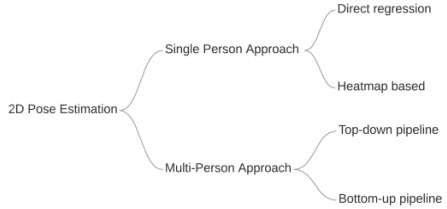
\includegraphics[scale=1]{gambar/taxonomy-pose-estimation.png}

  % Ubah dengan keterangan gambar yang diinginkan
  \caption{Taxonomi dari Pendekatan Estimasi Pose}
  \label{fig:pose-estimation}
\end{figure}

Estimasi pose adalah bidang yang sedang banyak diteliti sekarang, contohnya dalam menemukan makna dari sebuah pengenalan tindakan, pelacakan aktivitas, augmented reality, animasi, game, dan lain-lain.
Pendekatan yang ditawarkan juga berbeda tergantung dengan tujuannya agar memperoleh hasil yang lebih baik. Secara umum, estimasi pose dapat dibagi
menjadi dua kategori yaitu pendekatan satu-orang dan multi-orang seperti yang ditunjukkan
pada Gambar \ref{fig:pose-estimation}. Pendekatan satu-orang akan mendeteksi pose seseorang dalam gambar yang
diberikan (posisi orang tersebut) dan sejumlah keypoint, membuat hal ini menjadi seolah-olah
seperti masalah regresi. Di sisi lain, tujuan dari pendekatan multi-orang adalah untuk memecahkan masalah yang tidak dibatasi karena jumlah dan posisi orang di dalam gambar juga tidak
diketahui \parencite{romeo}.

Pendekatan satu-orang dibagi lagi menjadi dua berdasarkan metode prediksi \emph{keypoint}, melakukan regesi \emph{keypoint} secara langsung dari fitur-fitur yang ada (\emph{direct regression based framework}) atau dengan menghasilkan \emph{heatmap} dan menyimpulkan \emph{keypoint} dari \emph{heatmap} (\emph{heatmap based framework}) \parencite{romeo}.
\emph{Direct regression based framework} dapat dilakukan dengan berbagai macam cara, seperti yang telah dilakukan oleh Toshev dan Szegedy, model mereka menggunakan arsitektur sederhana dengan \emph{convolutional layer}, diikuti dengan \emph{dense layer} yang nantinya menghasilkan nilai \emph{keypoint} dalam \emph{(x,y)} \parencite{toshev2014}.
Ada juga metode yang memasukkan kembali kesalahan prediksi secara berulang-ulang, dan terbukti menghasilkan peningkatan akurasi yang signifikan seperti yang dilakukan oleh Luvizon et al. \parencite{carreira2015}.

Kemudian, untuk kerangka kerja berbasis \textit{heatmap}, dapat digunakan metode alternatif untuk menghasilkan \textit{heatmap} dari semua \emph{keypoint} pada gambar daripada langsung memprediksinya. Figur manusia akhir kemudian dibuat menggunakan teknik tambahan untuk mengetahui hubungan antara \emph{keypoint} atau sendi.
Dalam \parencite{chen2014}, para penulis mengusulkan model grafis dengan hubungan berpasangan untuk penggunaan adaptif dari pengukuran citra lokal. Selanjutnya, baik deteksi sendi maupun prediksi hubungan di antara mereka dapat dilakukan menggunakan pengukuran citra lokal tersebut.
\parencite{newell2016} merancang jaringan \emph{"stacked hourglass"} yang sangat mirip dengan arsitektur encoder-decoder dan didasarkan pada fase-fase berurutan dari pooling dan upsampling. Mereka mendemonstrasikan pentingnya proses pengolahan dari bawah ke atas yang berulang dengan supervisi menengah untuk meningkatkan efektivitas deteksi pose manusia.

Pendekatan multi-orang merupakan tugas yang lebih kompleks karena posisi dan jumlah orang dalam gambar tidak diketahui, sehingga kerangka kerja harus dapat mendeteksi \emph{keypoint} dan menggabungkannya dengan jumlah orang yang tidak diketahui.
Untuk mengatasi hal ini, dua pendekatan telah diusulkan: pendekatan top-down dan pendekatan bottom-up \parencite{romeo}. Dimulai dengan mendeteksi setiap orang yang ada dalam gambar, pendekatan top-down menciptakan \emph{bounding box}. Langkah selanjutnya adalah menggunakan setiap \emph{bounding box} yang teridentifikasi dan menerapkan pendekatan satu-orang.
Untuk setiap orang yang ditemukan, pendekatan satu-orang akan menghasilkan \emph{keypoint}, kemudian, seperti yang ditunjukkan pada Gambar \ref{fig:top-down-approach}, langkah-langkah tambahan diperlukan untuk p\emph{post-processing} dan peningkatan hasil akhir.

\begin{figure}[ht]
  \centering
  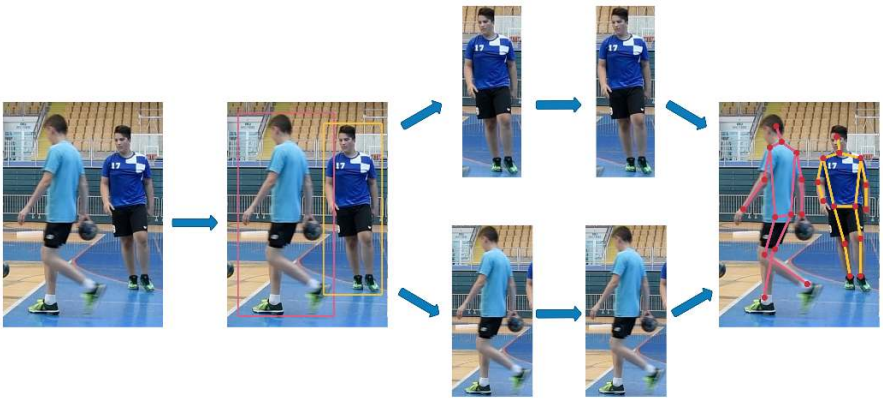
\includegraphics[scale=0.8]{gambar/top-down-approach.png}
  \caption{Alur Kerja Top-down pada Pendekatan Multi-orang untuk Estimasi Pose}
  \label{fig:top-down-approach}
\end{figure}

Dibandingkan dengan pendekatan top-down, pendekatan bottom-up bekerja secara kebalikannya. Pendekatan bottom-up dimulai dengan menemukan semua \emph{keypoints}, lalu dihubungkan ke setiap objek manusia, seperti yang terlihat pada Gambar \ref{fig:bottom-up-approach}.
Pendekatan bottom-up mungkin lebih cepat daripada pendekatan top-down karena tidak mendeteksi \emph{bounding box} manusia dan menjalankan estimasi pose untuk setiap orang.

\begin{figure}[ht]
  \centering
  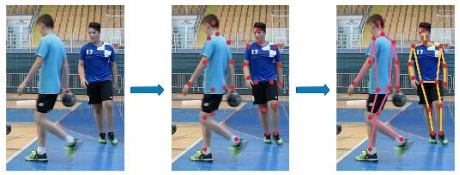
\includegraphics[scale=1.2]{gambar/bottom-up-approach.png}
  \caption{Alur Kerja Bottom-up pada Pendekatan Multi-orang untuk Estimasi Pose}
  \label{fig:bottom-up-approach}
\end{figure}

\subsection{Estimasi Pose Manusia}
\label{subsec:estimasi-pose-manusia}

Mengestimasi pose manusia merupakan salah satu hal yang paling menantang dalam visi komputer dengan tujuan untuk menentukan posisi atau lokasi spasial dari titik-titik tertentu pada tubuh seseorang (bagian tubuh/sendi) dari gambar atau video yang diberikan.
Pada dasarnya, ini adalah cara untuk memperoleh sekumpulan koordinat dengan mendefinisikan sendi-sendi tubuh manusia seperti pergelangan tangan, bahu, lutut, mata, telinga, pergelangan kaki, dan lengan, yang merupakan \emph{keypoint} dalam gambar atau video yang dapat menggambarkan pose seseorang. Kemudian, ketika sebuah gambar atau video diberikan sebagai input kepada model estimasi pose, model tersebut mengidentifikasi koordinat dari bagian-bagian tubuh dan sendi-sendi yang terdeteksi ini sebagai output, beserta dengan skor kepercayaan yang menunjukkan tingkat ketepatan estimasi tersebut.
Selama bertahun-tahun, topik utama dalam banyak deteksi objek klasik adalah deteksi orang. Dengan perkembangan terbaru dalam algoritma pembelajaran mesin, komputer sekarang dapat memahami bahasa tubuh manusia dengan melakukan deteksi pose dan pelacakan pose. Saat ini, teknologi ini telah mencapai titik di mana persyaratan perangkat keras untuk mengoperasikan dan akurasi deteksi membuatnya layak secara komersial.
Beberapa industri, termasuk keamanan, kecerdasan bisnis, kesehatan dan keselamatan, serta hiburan, akan sangat dipengaruhi oleh estimasi pose manusia. Salah satu contoh aplikasinya adalah kendaraan otonom di mana metode ini sudah terbukti layak. Komputer dapat mendeteksi dan memprediksi perilaku pejalan kaki dengan lebih komprehensif menggunakan deteksi pose manusia secara real-time, yang memungkinkan pengemudi untuk berkendara dengan lebih konsisten.

Estimasi pose pada manusia dapat dibagi menjadi dua teknik: Estimasi Pose 2D dan Estimasi Pose 3D.
Estimasi pose 2D adalah jenis estimasi pose yang dapat memperkirakan lokasi sendi-sendi tubuh dalam ruang 2D relatif terhadap data input (misalnya, gambar atau frame video). Lokasi tersebut direpresentasikan dengan koordinat X dan Y untuk setiap \emph{keypoint}. Di sisi lain, estimasi pose 3D mengubah gambar 2D menjadi objek 3D dengan memperkirakan dimensi Z tambahan pada prediksi. Estimasi pose 3D memungkinkan kita untuk memprediksi penempatan spasial yang akurat dari orang atau objek yang direpresentasikan.

Pada awalnya, tugas estimasi pose diperlakukan sebagai tugas inferensi berbasis bagian, dan terdapat dua kelompok model umum. Kelompok pertama disebut model tampilan, di mana fitur-fitur bagian tubuh pertama kali diekstraksi oleh deskriptor fitur seperti \emph{Histogram of Oriented Gradient}, kemudian bagian-bagian tubuh yang berbeda digabungkan bersama-sama.
Kelompok lainnya adalah model deformabel atau model struktural.
Kinerja model estimasi secara signifikan meningkat setelah \emph{deep convolutional networks} digunakan untuk estimasi pose. Awalnya, para peneliti berkonsentrasi pada masalah estimasi postur yang \emph{well-cropped single-person}, hal ini merupakan sub-tugas yang disederhanakan. Saat ini, situasi yang lebih sulit, termasuk estimasi pose dalam kerumunan, telah menjadi topik yang menarik berkat keberhasilan estimasi pose multi-orang yang lebih umum \parencite{song2021}.

\subsubsection{OpenPose}
\label{subsubsec:openpose}

OpenPose adalah \emph{open-source library} yang luas digunakan dan berpengaruh yang dikembangkan oleh Carnegie Mellon University dan Intel. Tujuannya adalah memberikan estimasi pose manusia yang akurat dan handal dengan mendeteksi dan melacak t\emph{keypoint} tubuh pada gambar dan video.
OpenPose menggunakan arsitektur khusus di mana gambar input diproses melalui \emph{state-of-the-art} CNN, seperti VGG-16 atau VGG-19. CNN ini menghasilkan tensor multidimensi yang dikenal sebagai \emph{feature maps}. \emph{Feature maps} ini kemudian dimasukkan ke dalam dua cabang pada \emph{Stage-1}.
Cabang pertama menghasilkan \emph{confidence maps} untuk bagian-bagian tubuh yang berbeda. Cabang kedua menghasilkan \emph{part affinity maps} (PAFs), yang merupakan vektor arah yang mewakili orientasi dari berbagai anggota tubuh.
Setelah \emph{Stage-1}, \emph{confidence maps}, PAFs, dan \emph{feature maps} dari CNN digabungkan dan digunakan sebagai input untuk \emph{Stage-2}. \emph{Stage-2} adalah replikasi dari \emph{Stage-1} dan bertujuan untuk menyempurnakan hasilnya. Dalam arsitektur OpenPose, mungkin ada beberapa tahap \emph{Stage-2} jika sumber daya komputasi masih tersedia. Hal ini dapat meningkatkan keakuratan prediksi pose manusia \parencite{cao2019}.
Gambar \ref{fig:openpose-architecture} menunjukkan arsitektur jaringan OpenPose, dengan blok yang memprediksi afinitas yang mengkodekan asosiasi antar bagian, ditunjukkan dengan warna biru lalu deteksi \emph{confidence maps}, ditunjukkan dengan warna cokelat muda.

\begin{figure}[ht]
  \centering
  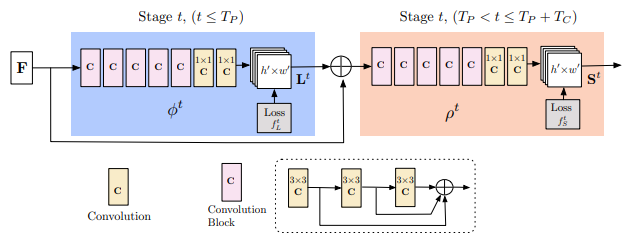
\includegraphics[scale=1.1]{gambar/openpose_architecture.png}
  \caption{Arsitektur OpenPose.}
  \label{fig:openpose-architecture}
\end{figure}

\subsubsection{MediaPipe Pose}
\label{subsec:mediapipepose}

MediaPipe Pose adalah \emph{open-source library} yang dikembangkan oleh Google, dirancang untuk estimasi pose manusia secara \emph{real-time}. Hal ini menggunakan model pembelajaran mesin dan teknik visi komputer untuk mendeteksi dan melacak landmark tubuh manusia dengan akurasi tinggi, memungkinkan pengaplikasiannya di berbagai bidang seperti robotika, analisis olahraga, kesehatan, dan \emph{augmented reality}.
Selama bertahun-tahun, MediaPipe Pose telah mengalami kemajuan yang signifikan, baik dari segi akurasi maupun performa. Pembaruan terbaru berfokus pada peningkatan kecepatan perpustakaan sehingga memungkinkan estimasi pose secara \emph{real-time} bahkan pada perangkat dengan sumber daya terbatas. Optimasi tersebut meliputi teknik kompresi model, peningkatan arsitektur jaringan, dan implementasi efisien pada akselerator perangkat keras. Selain itu, MediaPipe Pose sekarang juga mendukung estimasi pose multi-orang yang memungkinkan deteksi dan pelacakan beberapa individu secara bersamaan.
Dalam studi ini, MediaPipe Pose digunakan untuk mendapatkan estimasi koordinat sendi manusia 2D pada setiap frame gambar. Hal ini membangun alur kerja dan memproses data kognitif dalam bentuk video menggunakan pembelajaran mesin. MediaPipe Pose menggunakan BlazePose yang mengekstraksi 33 landmark 2D pada tubuh manusia seperti yang ditunjukkan pada Gambar \ref{fig:mediapipe-landmark}. BlazePose adalah arsitektur pembelajaran mesin yang ringan dan mencapai performa real-time pada ponsel dan PC dengan inferensi CPU.
Ketika menggunakan koordinat yang ternormalisasi untuk estimasi pose, kita perlu mengalikannya dengan lebar atau tinggi gambar untuk mendapatkan nilai piksel yang sebenarnya

\begin{figure}[ht]
  \centering
  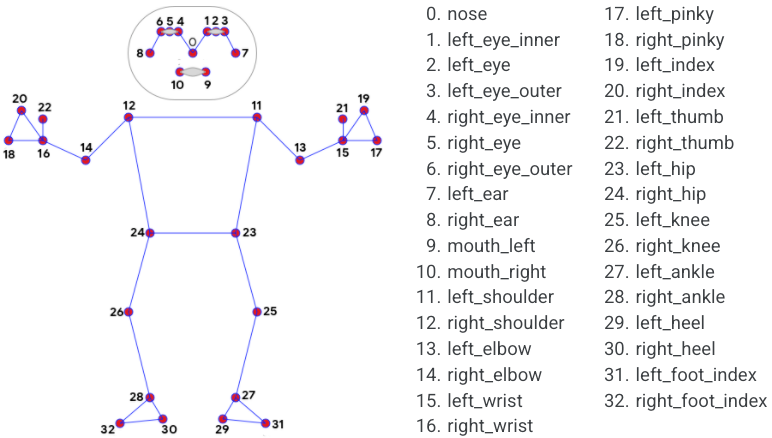
\includegraphics[scale=0.4]{gambar/mediapipe_landmark.png}
  \caption{Definisi Landmarks pada MediaPipe Pose.}
  \label{fig:mediapipe-landmark}
\end{figure}

BlazePose terdiri dari dua komponen utama: detektor dan pelacak. Detektor bertanggung jawab untuk mendeteksi keberadaan seseorang dalam gambar input atau frame video. Detektor ini akan menemukan tubuh orang dalam gambar dan memberikan set awal untuk \emph{keypoints} pose, dengan kata lain, menemukan \emph{region of interest} (ROI) pose dalam frame.
Detektor menggunakan arsitektur j\emph{convolutional neural network} (CNN) untuk mengekstrak fitur dari input dan membuat prediksi tentang keberadaan dan lokasi tubuh orang tersebut. Pelacak kemudian memprediksi semua 33 \emph{keypoints} pose dari ROI ini. Perlu dicatat bahwa detektor hanya dijalankan pada frame pertama dalam kasus video. Untuk frame selanjutnya, cara untuk mendapatkan ROI berasal dari \emph{keypoints} pose frame sebelumnya \parencite{url:BlazePose}.

\subsubsection{YOLO-pose}
\label{subsubsec:yolopose}

YOLO-pose adalah pendekatan single-shot seperti pendekatan bottom-up lainnya. Namun, YOLO-pose tidak menggunakan \emph{heatmap}. Sebaliknya, YOLO-pose menghubungkan semua \emph{keypoint} pose seseorang dengan anchor. Gambar \ref{fig:YOLO-pose-architecture} menggambarkan keseluruhan arsitektur  
dengan beberapa \emph{keypoint head} untuk estimasi pose. Detektor manusia yang paling canggih dalam hal kompleksitas dan akurasi adalah YOLOv5. Oleh karena itu, YOLOv5 dipilih sebagai dasar pembuatan YOLO-pose ini.
Fokus utama YOLOv5 adalah pengenalan 80 objek kelas COCO, dengan \emph{box head} yang memprediksi 85 elemen tiap anchor. Terdapat tiga anchor dengan bentuk yang berbeda untuk setiap lokasi grid \parencite{maji2022yolopose}.

\begin{figure}[ht]
  \centering
  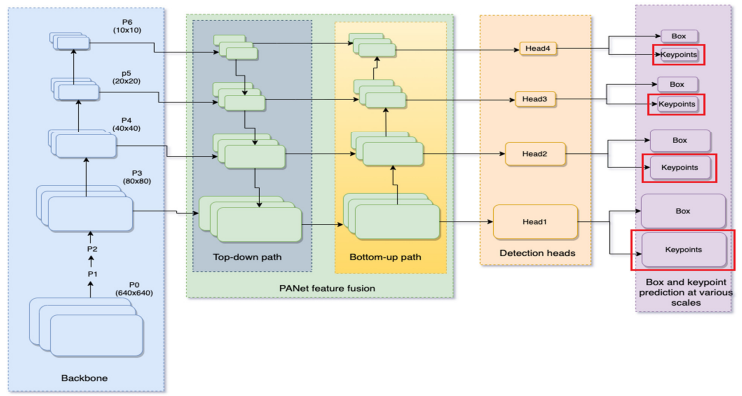
\includegraphics[scale=0.9]{gambar/yolo-architecture.png}
  \caption{Arsitektur YOLO-pose.}
  \label{fig:YOLO-pose-architecture}
\end{figure}
\newpage
Untuk estimasi pose manusia, hal ini menjadi masalah deteksi orang tunggal dengan setiap orang memiliki 17 \emph{keypoint} terkait, masing-masingnya berisi lokasi dan tingkat kepercayaan: \emph{{x, y, conf}}.
Oleh karena itu, total ada 51 elemen untuk 17 \emph{keypoint} yang terkait dengan sebuah anchor. Sebagai hasilnya, \emph{keypoint head} memprediksi 51 elemen dan \emph{box head} memprediksi enam elemen untuk setiap anchor.
Untuk sebuah anchor dengan n \emph{keypoint}, prediksi keseluruhan vektor didefinisikan sebagai:
\begin{equation}
  \label{eq:yoloresult}
  P_v = \bigl\{ C_x, C_y, W, H, box_{conf}, class_{conf}, K_x^1, K_y^1, K_{conf}^1, ..., ..., ..., K_x^n, K_y^n, K_{conf}^n \bigr\}
\end{equation}

Tingkat kepercayaan sebuah \emph{keypoint} dilatih berdasarkan tanda visibilitas \emph{keypoint}. Nilai kepercayaan \emph{ground truth} bernilai satu jika \emph{keypoint} tersebut terlihat atau terhalang. Jika \emph{keypoint} berada di luar bidang pandang, nilainya nol.
YOLO-Pose menggunakan CSP-darknet53 \parencite{wang2020} sebagai \emph{backbone} dan PANet \parencite{liu2018} untuk menggabungkan fitur dari skala yang berbeda yang berasal dari \emph{backbone} tersebut.
Gambar input masuk melalui \emph{backbone} darknetcsp yang menghasilkan \emph{feature map} dengan skala yang berbeda-beda {P3, P4, P5, P6}.
PAnet digunakan untuk menggabungkan \emph{feature map} ini di berbagai skala dan outputnya diberikan ke \emph{detection head}.
Akhirnya, setiap \emph{head head} bercabang menjadi \emph{box head} dan \emph{keypoint head} \parencite{maji2022yolopose}.

\subsection{Estimasi Pose Robot \emph{Humanoid}}
\label{subsec:estimasi-pose-robot-humanoid}

Robot \emph{humanoid} dan manusia memiliki bentuk fisik yang mirip, di mana hal ini memiliki kelebihan dan kekurangannya masing-masing. Di satu sisi, hal ini memungkinkan kita untuk menggunakan metode estimasi pose yang awalnya ditujukan untuk manusia kepada robot, tetapi di sisi lain, hal ini juga mempersulit kita untuk membedakan antara manusia dan robot humanoid \parencite{amini2021}.
Seperti yang dijelaskan di Bagian \ref{subsec:estimasi-pose}, secara umum, upaya untuk mengatasi masalah estimasi pose sangat bergantung pada jumlah orang (satu orang atau lebih dari satu), untuk  multi-orang dapat dibagi lagi menjadi pendekatan top-down atau bottom-up.
Dalam pendekatan top-down, tahap awal adalah mengidentifikasi setiap individu dalam gambar lalu mengimplementasikan estimasi pose untuk tiap individu.
Salah satu kelemahan pendekatan ini adalah performa model sangat terkait dengan performa detektor orang. Waktu eksekusinya sangat terpengaruh oleh jumlah orang yang ada karena estimasi pose satu-orang dijalankan untuk setiap deteksi. Karena biaya komputasinya yang meningkat secara linear seiring dengan peningkatan jumlah orang, sering kali performanya tidak real-time \parencite{amini2021}.

Di sisi lain, teknik bottom-up tidak bergantung pada jumlah orang dalam gambar karena mereka secara simultan mengidentifikasi sendi-sendi tubuh dan mengklasifikasikannya ke dalam individu-individu. Pengelompokkan dengan akurat dari \emph{keypoint} yang terdeteksi secara real-time merupakan salah satu isu fundamental dalam metode bottom-up.
Metode terkini mengatur \emph{keypoint} yang teridentifikasi menjadi individu yang terpisah menggunakan algoritma \emph{greedy}. Selain itu, dibandingkan dengan metode top-down, efektivitas metode bottom-up lebih dipengaruhi oleh berbagai skala orang dalam gambar yang diberikan. Penelitian sebelumnya telah mengandalkan ukuran input resolusi tinggi \parencite{papandreou2018} atau metode pencarian skala \parencite{cao2019} untuk mengatasi masalah ini. Namun, waktu inferensi bertambah akibat hal tersebut.
Metode yang efisien waktu memprediksi \emph{keypoint} dengan resolusi yang lebih tinggi diperkenalkan oleh Cheng et al. \parencite{cheng2020} sehingga dapat mempersempit kesenjangan performa antara model bottom-up dan top-down.

Terdapat tiga Model estimasi pose untuk robot humanoid yang kami latih ulang menggunakan dataset baru. Dua diantaranya menggunakan pendekatan bottom-up dan satu menggunakan pendekatan top-down. Penjelasan lebih rinci tentang setiap model terdapat pada bagian berikutnya.

\subsubsection{Model NimbRo}
\label{subsubsec:nimbromodel}

Model NimbRo memilih untuk menggunakan arsitektur yang mirip dengan NimbRo-Net dan NimbRo-Net2 karena memiliki hasil yang positif.
Model mereka merupakan jaringan \emph{encoder-decoder} dengan gambar \emph{input} RGB berdimensi \emph{w x h}. Alih-alih menggunakan \emph{decoder} untuk membuat ekstraktor fitur yang unggul, mereka mengamati bahwa lebih penting untuk menggunakan \emph{encoder} yang lebih dalam.
Model ResNet yang telah dilatih sebelumnya \parencite{he2016} digunakan sebagai \emph{encoder}, dan lapisan \emph{fully connected} serta \emph{global average pooling} di bagian akhir telah dihilangkan.
Layer pertama adalah konvolusi 7 x 7 dengan langkah 2, diikuti oleh layer \emph{max-pooling}. Empat modul lainnya dari \emph{encoder} adalah blok residual di mana memiliki resolusi yang lebih rendah dan kedalaman yang lebih tinggi seiring dengan peningkatan jumlah modul.
Tergantung pada arsitektur ResNet yang dipilih, setiap blok residual terdiri dari dua atau tiga layer konvolusi, diikuti oleh normalisasi batch, aktivasi ReLU, dan koneksi shortcut. Layer awal memiliki informasi spasial yang lebih detail,
sedangkan layer terakhir mengandung informasi semantik yang lebih banyak \parencite{amini2021}.

\begin{figure}[ht]
  \centering
  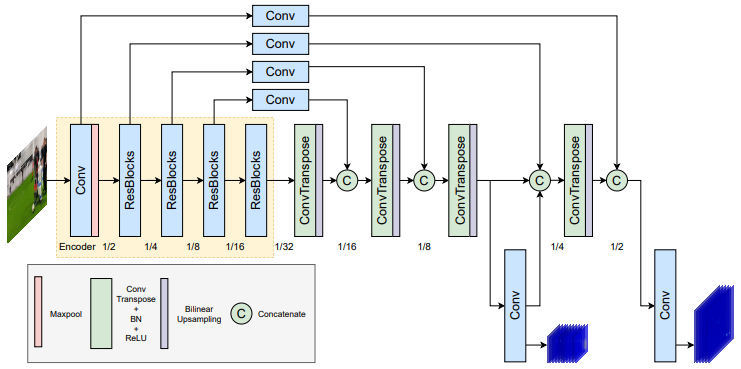
\includegraphics[scale=0.9]{gambar/nimbro-architecture.png}
  \caption{Arsitektur Model NimbRo}
  \label{fig:nimbro-model-architecture}
\end{figure}

Pada bagian \emph{decoder}, mereka menggunakan koneksi lateral dari bagian-bagian yang berbeda pada encoder, yang memungkinkan model untuk mempertahankan informasi dengan resolusi tinggi. Mereka menerapkan konvolusi 1 x 1 untuk menghasilkan jumlah saluran yang tetap untuk setiap koneksi lateral.
Jaringan \textit{decoder} memiliki struktur piramida fitur yang terdiri dari empat modul. Keluaran dari tingkat sebelumnya dimasukkan ke dalam konvolusi 3 x 3 pada setiap tingkat piramida, diikuti oleh \textit{upsampling bilinear} untuk menghasilkan fitur resolusi yang lebih tinggi.
Fitur dari koneksi lateral yang sesuai akan digabungkan dengan fitur dari sampel yang telah di-\textit{upsample}. ReLU dan normalisasi batch digunakan seperti pada \textit{encoder} untuk mendapatkan output akhir modul tersebut.
Seperti pada Gambar \ref{fig:nimbro-model-architecture}, model ini memprediksi \textit{heatmap} untuk kedua \textit{keypoint} dan anggota tubuh dengan skala 1/4, dan hanya \textit{heatmap} untuk \textit{keypoint} dengan skala 1/2, di mana setiap skala disupervisi dengan \textit{intermediate loss} \parencite{amini2021}.
Untuk metrik evaluasi yang digunakan adalah metrik \textit{Object Keypoint Similarity} (OKS) dari dataset \textit{keypoint} COCO \parencite{ronchi2017}.
Metrik evaluasi yang digunakan adalah sebagai berikut: AP (rata-rata presisi dari 10 batas OKS = [0,50:0,05:0,95]), AP50 (presisi rata-rata pada batas OKS = 0,50), AP75, APM untuk robot dengan skala \textit{medium}, APL untuk skala \textit{large}, dan AR (rata-rata recall dari 10 batas OKS) \parencite{amini2021}.

\subsubsection{Keypoint RCNN}
\label{subsubsec:rcnn}

Arsitektur Keypoint RCNN merupakan modifikasi dari Mask-RCNN. Mereka hanya berbeda dalam ukuran output, dan cara \textit{keypoint} dikodekan dalam masker \textit{keypoint}. Mask R-CNN sendiri dibangun berdasarkan Faster R-CNN,
selain dari jaringan dasar bersama dan FPN (\textit{Feature Pyramid Networks}), Mask R-CNN juga secara paralel menambahkan cabang baru untuk memprediksi \textit{object mask} pada cabang pengenalan \textit{bounding box}.
Jaringan ini juga dapat dimodifikasi dengan mudah untuk melaksanakan tugas tambahan seperti Keypoint RCNN untuk deteksi \textit{keypoint} pada manusia. \textit{Keypoint head} dari Keypoint R-CNN sangat mirip dengan \textit{mask head} pada Mask R-CNN. 
\textit{Mask head} memperoleh resolusi output 28 x 28 melalui empat lapisan konvolusi 3 x 3 dengan kanal sebesar 256 yang diikuti oleh lapisan \textit{upsampling}, dan akhirnya menggunakan lapisan konvolusi untuk membuat dimensinya konsisten dengan kategori objek.
Di sisi lain, \textit{keypoint head} memperoleh resolusi output 56 x 56 melalui delapan lapisan konvolusi 3 x 3 dengan 512 kanal dan diikuti oleh dua lapisan \textit{upsampling} \parencite{zhang2021}.

\begin{figure}[ht]
  \centering
  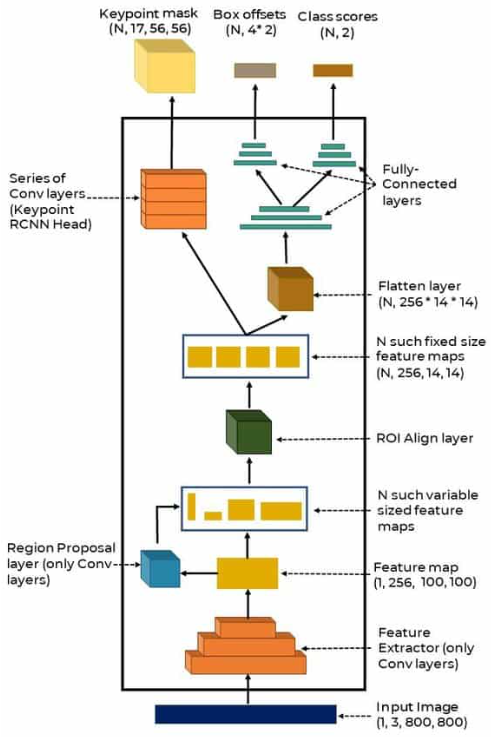
\includegraphics[scale=0.8]{gambar/keypoint-rcnn-arch.png}
  \caption{Arsitektur Keypoint RCNN}
  \label{fig:keypoint-rcnn-architecture}
\end{figure}


\subsection{\textit{Robot Operating System} 2 (ROS 2)}
\label{subsec:ros2}

\textit{Robot Operating System} (ROS) \parencite{quigley} merupakan sebuah \textit{open source} \textit{robotics middleware} yang digunakan untuk membantu pengembangan sistem yang ada pada robot. Fitur utama
pada ROS adalah desain sistem di mana data yang diterima maupun dikirim ke setiap komponen yang ada pada robot dilakukan secara terabstraksi dengan adanya \textit{hardware abstraction}. Melalui hal tersebut, algoritma yang ada pada suatu program
dapat digunakan pada robot yang berbeda, terlepas dari perbedaan perangkat yang ada di setiap robot.
ROS menggunakan \textit{graph architecture} untuk memungkinkan terjadinya \textit{hardware abstraction} sehingga suatu \textit{node} dapat berkomunikasi dengan \textit{node} lain melalui sebuah \textit{topic} yang sama.
\textit{Hardware abstraction} tersebut terbentuk dengan menggunakan \textit{topic} yang memiliki nama dan struktur data yang sama yang merepresentasikan jenis komponen yang dimiliki suatu robot.
Nantinya, setiap \textit{node} dapat menerima maupun mengirimkan data melalui \textit{topic} tersebut, terlepas dari asal data tersebut.

Pada ROS sudah terdapat beragam \textit{tools} yang dapat membantu pengembangan sistem yang ada pada robot seperti \textit{command-line} yang membantu dalam \textit{debugging} program,
konfigurasi parameter secara dinamis ketika program sedang dijalankan, \textit{monitoring} data internal yang ada pada robot secara visual,
dan lain-lain. Selain itu, dengan \textit{package management} pada ROS, setiap orang bisa menggunakan \textit{package} yang sudah
ada maupun menambahkan \textit{package} baru untuk mempermudah pengembangan lebih lanjut dari suatu robot, tanpa perlu membuat keseluruhan sistem dari awal.
Generasi kedua dari \textit{Robot Operating System} (ROS 2) merupakan versi lanjutan dari ROS yang mengusung reliabilitas dan performa untuk penggunaan \textit{real-time} pada robot tetapi juga masih mendukung fitur yang dimiliki oleh ROS sebelumnya. Berbeda dengan
pendahulunya yang menggunakan TCPROS/UDPROS sebagai sistem komunikasi yang digunakan di setiap node, ROS 2 menggunakan \textit{Data Distribution Service} (DDS), standar industri
untuk sistem komunikasi \textit{real-time} dan \textit{end-to-end middleware}. Dengan penggunaan DDS tersebut, ROS 2 akan lebih terfokus pada
penggunaan \textit{middleware} di bidang robotika, sedangkan komunikasi tingkat rendah yang dilakukan antar \textit{node} akan dikembalikan kepada implementasi DDS yang digunakan.

\subsubsection{\textit{ROS 2 Node}}
\label{subsubsec:ros2node}

\textit{ROS 2 node} merupakan komponen utama dari \textit{graph architecture} pada ROS 2. \textit{ROS 2 node} umumnya digunakan untuk
merepresentasikan suatu proses tunggal yang ada pada robot, seperti untuk mengakses motor, mengolah gambar, dan sebagainya.
Setiap \textit{node} dapat berkomunikasi dengan \textit{node} lain melalui dua cara, seperti yang terlihat pada Gambar \ref{fig:ros2node}, sebuah \textit{node} dengan \textit{publisher} dapat mengirimkan sebuah data melalui
\textit{topic} yang nantinya akan diterima oleh \textit{node} lain dengan \textit{subscriber} yang terhubung dengan topic tersebut. Selain itu, sebuah \textit{node}
dengan \textit{service client} juga dapat mengirimkan sebuah data \textit{request} melalui \textit{service} yang nantinya akan diolah dan dikirim balik dalam
bentuk data \textit{response} oleh \textit{node} lain yang memiliki \textit{service server} yang terhubung dengan \textit{service} tersebut.
Proses komunikasi antar-\textit{node} tersebut dilakukan secara terabstraksi, di mana suatu node akan mengirimkan data ke suatu \textit{topic} maupun \textit{service}, terlepas dari apakah data tersebut
akan diterima oleh \textit{node} lain atau tidak. Setiap \textit{node} nantinya cukup mengirimkan data ke \textit{topic} atau \textit{service} dengan nama dan tipe
\textit{interface} yang sesuai agar data tersebut dapat dikirimkan secara terabstraksi ke \textit{node} lain.
Selain \textit{topic} dan \textit{service}, ROS 2 juga mengenal bentuk lain dari jalur komunikasi antar-\textit{node} yang disebut sebagai \textit{action}. Tetapi karena hal ini tidak digunakan pada penelitian ini maka kita tidak akan mendiskusikannya lebih lanjut. 
\begin{figure}[ht]
  \centering
  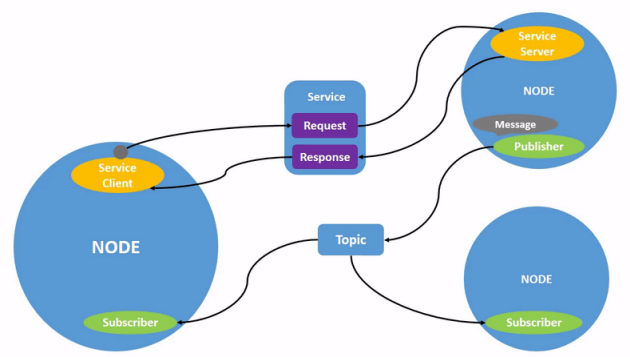
\includegraphics[scale=0.9]{gambar/ros2_node.png}
  \caption{Diagram Komunikasi Antar-\textit{node} Melalui \textit{Topic} dan \textit{Service} pada ROS 2}
  \label{fig:ros2node}
\end{figure}

\subsubsection{RQt}
\label{subsubsec:rqt}

RQt merupakan \textit{framework} \textit{GUI} berbasis Qt yang digunakan untuk mengimplementasikan \textit{tools} dalam mengatur node yang
ada pada ROS 2 \parencite{url:rqt}. RQt memiliki fungsi yang relatif sama dengan \textit{ROS 2 CLI}, yakni untuk keperluan \textit{debugging} pada sistem
komunikasi yang ada pada ROS 2, namun RQt ini bekerja secara visual dalam bentuk GUI. Seperti yang ditunjukkan pada Gambar \ref{fig:rqtgraph}, RQt memiliki \textit{tools} bernama rqt graph (ROS Graph) yang dapat digunakan untuk melihat hubungan yang ada pada
setiap \textit{node} dalam bentuk \textit{topic}, \textit{service}, maupun \textit{action}. Selain \textit{tools} bawaan yang sudah tersedia, \textit{tools} berbasis GUI
pada RQt juga bisa dibuat sendiri serta diubah sesuai dengan kebutuhan. Perubahan tersebut dapat dilakukan melalui \textit{plugin} khusus untuk RQt. Nantinya
\textit{plugin} tersebut dapat disematkan pada \textit{tools} RQt yang dikembangkan dan secara langsung dapat digunakan untuk mengakses sistem komunikasi yang ada pada ROS 2
\begin{figure}[ht]
  \centering
  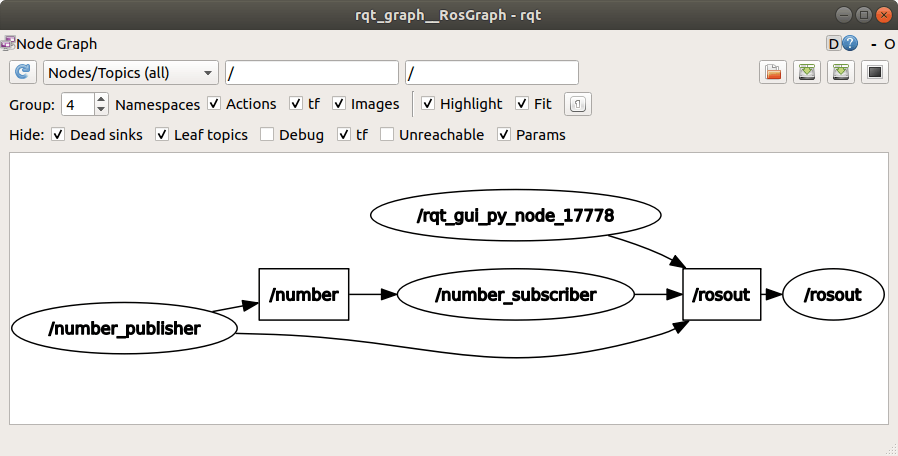
\includegraphics[scale=0.45]{gambar/rqt_graph.png}
  \caption{Contoh Tampilan Rqt Graph (\textit{ROS Graph})}
  \label{fig:rqtgraph}
\end{figure}


\subsection{ Metrik Evaluasi}
\label{subsec:evaluation-metrics}

Metrik evaluasi adalah ukuran yang digunakan untuk menilai kinerja dan efektivitas model pembelajaran mesin atau visi komputer. Metrik ini memberikan wawasan kuantitatif tentang seberapa baik model tersebut berkinerja dalam berbagai aspek seperti presisi, \textit{recall}, dan lain-lain.

\subsubsection{Presisi}
\label{subsubsec:precision}

Presisi merupakan metrik yang digunakan untuk mengukur rasio prediksi positif yang benar (\textit{true positives}) dari semua prediksi positif (\textit{true positives} + \textit{false positives}).
Dengan kata lain, metrik ini mengukur kemampuan model untuk menghindari positif palsu. Presisi yang lebih tinggi menunjukkan jumlah positif palsu yang lebih sedikit dan tingkat kesalahan yang lebih rendah dalam mengklasifikasikan instansi negatif sebagai positif.
Nilai presisi berkisar antara 0 dan 1. Rumus \ref{eq:precision} adalah persamaan untuk menghitung presisi.

\begin{equation}
  \label{eq:precision}
  \frac{TP}{(TP+FP)}
\end{equation}

\subsubsection{Recall}
\label{subsubsec:recall}

\textit{Recall} merupakan metrik yang digunakan untuk mengukur rasio dari data positif yang benar (\textit{true positives}) yang ditemukan dari seluruh data positif (\textit{true positives} + \textit{false negatives}).
Nilai \textit{recall} yang lebih tinggi menunjukkan jumlah negatif palsu yang lebih sedikit dan tingkat kesalahan yang lebih rendah dalam mengklasifikasikan instansi positif sebagai negatif.
Nilai \textit{recall} berkisar antara 0 dan 1. Rumus \ref{eq:recall} adalah persamaan untuk menghitung \textit{recall}.
\begin{equation}
  \label{eq:recall}
  \frac{TP}{(TP+FN)}
\end{equation}